% appendices/appendix-a-quantum-primer.tex
% Appendix A: Primer on Quantum Information Processing

\chapter{Primer on Quantum Information Processing}

This appendix provides essential background on quantum computing concepts for readers less familiar with the field. Understanding these fundamentals is crucial for appreciating the quantum clustering algorithms discussed in this report.

\section{From Classical to Quantum}

Classical computers process information using bits that exist in one of two states: 0 or 1. Quantum computers use quantum bits, or \textit{qubits}, which can exist in superpositions of both states simultaneously. This fundamental difference enables quantum computers to process information in ways that are impossible for classical systems.

\begin{keyconceptbox}[Classical vs. Quantum]
The key distinctions between classical and quantum computing:
\begin{itemize}
    \item \textbf{Classical bits:} Deterministic states (0 or 1)
    \item \textbf{Qubits:} Probabilistic superposition of states
    \item \textbf{Classical operations:} Boolean logic gates
    \item \textbf{Quantum operations:} Unitary transformations preserving probability
\end{itemize}
\end{keyconceptbox}

\section{Quantum Bits (Qubits)}
\label{sec:qubits}

The fundamental unit of quantum information is the quantum bit, or qubit. Unlike classical bits that exist definitively in state 0 or 1, qubits can exist in quantum superposition states.

\begin{definitionbox}[Qubit State]
A qubit state $\ket{\psi}$ can be written as:
\begin{equation}
    \ket{\psi} = \alpha\ket{0} + \beta\ket{1}
\end{equation}
where $\alpha, \beta \in \mathbb{C}$ are complex amplitudes satisfying $|\alpha|^2 + |\beta|^2 = 1$.
\end{definitionbox}

The state can be visualized on the Bloch sphere using the parametrization:
\begin{equation}
    \ket{\psi} = \cos\frac{\theta}{2}\ket{0} + e^{i\phi}\sin\frac{\theta}{2}\ket{1}
\end{equation}

where $\theta \in [0, \pi]$ and $\phi \in [0, 2\pi)$.

\textbf{Multiple qubits:} A system of $n$ qubits exists in a $2^n$-dimensional Hilbert space:
\begin{equation}
    \ket{\psi} = \sum_{i=0}^{2^n-1} \alpha_i \ket{i}
\end{equation}

This exponential growth in state space is the source of quantum computational power.

\section{Superposition}
\label{sec:superposition}

Superposition is the principle that a quantum system can exist in multiple states simultaneously until measured. For $n$ qubits, a quantum system can represent $2^n$ states simultaneously.

\begin{definitionbox}[Quantum Superposition]
A quantum state $\ket{\psi}$ is in superposition when it cannot be expressed as a single basis state, but rather as a linear combination:
\begin{equation}
    \ket{\psi} = \sum_{i=0}^{2^n-1} \alpha_i \ket{i}, \quad \text{where } \sum_{i} |\alpha_i|^2 = 1
\end{equation}
\end{definitionbox}

This exponential scaling is the foundation of \textbf{quantum parallelism}. A quantum algorithm can process all $2^n$ states in parallel, potentially achieving exponential speedups for certain problems.

\begin{tipbox}[Relevance to Clustering]
In clustering, superposition could allow simultaneous evaluation of a pixel's distance to all cluster centroids, potentially reducing the number of operations required. Instead of computing $k$ distances sequentially, a quantum state can encode all distance comparisons in superposition.
\end{tipbox}

\section{Quantum Gates}
\label{sec:quantum-gates}

Quantum computation is performed through quantum gates, which are unitary transformations on qubit states. A transformation $U$ is unitary if $U^\dagger U = UU^\dagger = I$.

\begin{notebox}[Common Single-Qubit Gates]
\begin{itemize}
    \item \textbf{Pauli-X (NOT gate):} $X = \begin{pmatrix} 0 & 1 \\ 1 & 0 \end{pmatrix}$ — Bit flip
    \item \textbf{Pauli-Y:} $Y = \begin{pmatrix} 0 & -i \\ i & 0 \end{pmatrix}$ — Bit and phase flip
    \item \textbf{Pauli-Z:} $Z = \begin{pmatrix} 1 & 0 \\ 0 & -1 \end{pmatrix}$ — Phase flip
    \item \textbf{Hadamard (H):} $H = \frac{1}{\sqrt{2}}\begin{pmatrix} 1 & 1 \\ 1 & -1 \end{pmatrix}$ — Creates superposition
    \item \textbf{Phase gates (S, T):} Apply phase shifts of $\pi/2$ and $\pi/4$ respectively
    \item \textbf{Rotation gates ($R_x$, $R_y$, $R_z$):} Parameterized rotations around Bloch sphere axes
\end{itemize}
\end{notebox}

\textbf{Two-qubit gates:} Multi-qubit gates enable entanglement and conditional operations:

\begin{itemize}
    \item \textbf{CNOT (Controlled-NOT):} Fundamental entangling gate—flips target qubit if control is $\ket{1}$
    \item \textbf{SWAP:} Exchanges the states of two qubits
    \item \textbf{Controlled-phase gates:} Apply conditional phase shifts based on control qubit state
\end{itemize}

The CNOT gate matrix representation:
\begin{equation}
    \text{CNOT} = \begin{pmatrix} 1 & 0 & 0 & 0 \\ 0 & 1 & 0 & 0 \\ 0 & 0 & 0 & 1 \\ 0 & 0 & 1 & 0 \end{pmatrix}
\end{equation}

\section{Quantum Entanglement}
\label{sec:entanglement}

Entanglement is a uniquely quantum phenomenon where the states of multiple qubits become correlated in ways that cannot be described classically.

\begin{definitionbox}[Bell States]
The four maximally entangled two-qubit states are:
\begin{align}
    \ket{\Phi^+} &= \frac{1}{\sqrt{2}}(\ket{00} + \ket{11}) \\
    \ket{\Phi^-} &= \frac{1}{\sqrt{2}}(\ket{00} - \ket{11}) \\
    \ket{\Psi^+} &= \frac{1}{\sqrt{2}}(\ket{01} + \ket{10}) \\
    \ket{\Psi^-} &= \frac{1}{\sqrt{2}}(\ket{01} - \ket{10})
\end{align}
\end{definitionbox}

Entanglement is a resource for quantum algorithms, enabling correlations that speed up computation. Measuring one qubit immediately determines the state of the other, regardless of the distance between them—a property Einstein famously called ``spooky action at a distance.''

\begin{tipbox}[Relevance to Clustering]
Entanglement could capture complex correlations between pixels, potentially enabling more sophisticated similarity measures and better representation of spatial relationships in images. Entangled qubits can encode non-local dependencies that are difficult to represent classically.
\end{tipbox}

\section{Quantum Measurement}
\label{sec:measurement}

Measurement is the process of extracting classical information from a quantum state. Upon measurement, a quantum state \textit{collapses} to one of the basis states with probability determined by the amplitudes.

\begin{definitionbox}[Measurement Postulate]
For a state $\ket{\psi} = \sum_i \alpha_i \ket{i}$, measurement in the computational basis yields outcome $i$ with probability:
\begin{equation}
    P(i) = |\alpha_i|^2
\end{equation}
After measurement, the state collapses to $\ket{i}$.
\end{definitionbox}

\begin{warningbox}[Measurement Problem]
Measurement destroys superposition, collapsing the state to a single outcome. This means quantum algorithms must be carefully designed to extract useful information before decoherence occurs. The art of quantum algorithm design lies in arranging interference patterns so that correct answers have high measurement probability.
\end{warningbox}

\section{Quantum Algorithms}

Several quantum algorithms provide speedups relevant to clustering:

\subsection{Grover's Search Algorithm}

Grover's algorithm searches an unstructured database of $N$ items in $O(\sqrt{N})$ queries, compared to $O(N)$ classically.

\textbf{Application to clustering:} Finding the nearest centroid among $k$ centroids can be accelerated from $O(k)$ to $O(\sqrt{k})$.

\subsection{Quantum Phase Estimation}

Given a unitary $U$ and its eigenstate $\ket{u}$ with $U\ket{u} = e^{2\pi i\phi}\ket{u}$, phase estimation determines $\phi$ to $n$ bits of precision using $O(2^n)$ applications of controlled-$U$.

\textbf{Application to clustering:} Finding eigenvalues of the Laplacian matrix for spectral clustering.

\subsection{HHL Algorithm for Linear Systems}

The Harrow-Hassidim-Lloyd (HHL) algorithm solves $A\mathbf{x} = \mathbf{b}$ in time $O(\text{poly}(\log N, \kappa))$ where $\kappa$ is the condition number of $A$.

\textbf{Application to clustering:} Computing matrix inversions and solving linear systems that arise in various clustering formulations.

\subsection{Shor's Algorithm}

Shor's algorithm factors large integers exponentially faster than known classical algorithms, reducing the complexity from sub-exponential to polynomial time.

\textbf{Significance:} Demonstrates that quantum computers can solve problems believed to be intractable classically, with major implications for cryptography.

\subsection{Quantum Fourier Transform (QFT)}

The Quantum Fourier Transform is exponentially faster than the classical Fast Fourier Transform (FFT):

\begin{equation}
    \text{QFT}\ket{j} = \frac{1}{\sqrt{N}} \sum_{k=0}^{N-1} e^{2\pi ijk/N} \ket{k}
\end{equation}

\textbf{Application to clustering:} QFT is a subroutine in many quantum algorithms including phase estimation, which underlies quantum spectral clustering methods.

\subsection{Variational Quantum Eigensolver (VQE)}

VQE is a hybrid quantum-classical algorithm designed for NISQ devices. It finds ground states of quantum systems by:
\begin{enumerate}
    \item Preparing a parameterized quantum state (ansatz)
    \item Measuring the expected energy
    \item Classically optimizing the parameters to minimize energy
\end{enumerate}

\textbf{Application to clustering:} VQE can optimize clustering objectives encoded as Hamiltonians, making it suitable for near-term quantum hardware.

\begin{tipbox}
While these algorithms offer theoretical speedups, they often require fault-tolerant quantum computers. NISQ-era implementations typically use variational approximations (like VQE and QAOA) that trade optimality for noise resilience.
\end{tipbox}

\section{Hamiltonians and Quantum Dynamics}
\label{sec:hamiltonian}

The Hamiltonian is the central mathematical object that governs quantum systems. Understanding Hamiltonians is essential for quantum annealing and variational quantum algorithms.

\subsection{What is a Hamiltonian?}

\begin{definitionbox}[Hamiltonian]
The \textbf{Hamiltonian} $H$ is a Hermitian operator that represents the total energy of a quantum system. Its eigenvalues correspond to the possible energy levels, and its eigenstates are the stationary states of the system:
\begin{equation}
    H \ket{\psi_n} = E_n \ket{\psi_n}
\end{equation}
where $E_n$ is the energy of eigenstate $\ket{\psi_n}$.
\end{definitionbox}

\textbf{Key properties:}
\begin{itemize}
    \item \textbf{Hermiticity:} $H = H^\dagger$ ensures real eigenvalues (energies are real numbers)
    \item \textbf{Ground state:} The lowest-energy eigenstate $\ket{\psi_0}$ with energy $E_0$
    \item \textbf{Spectral gap:} The energy difference $\Delta = E_1 - E_0$ between ground and first excited state
\end{itemize}

\subsection{Time Evolution}

The Hamiltonian determines how quantum states evolve in time through the Schrödinger equation:

\begin{definitionbox}[Schrödinger Equation]
The time evolution of a quantum state is governed by:
\begin{equation}
    i\hbar \frac{\partial}{\partial t} \ket{\psi(t)} = H \ket{\psi(t)}
\end{equation}
For time-independent $H$, the solution is:
\begin{equation}
    \ket{\psi(t)} = e^{-iHt/\hbar} \ket{\psi(0)}
\end{equation}
where $e^{-iHt/\hbar}$ is the \textbf{time evolution operator}.
\end{definitionbox}

\begin{notebox}
In quantum computing, we often set $\hbar = 1$ for simplicity. The evolution operator $U(t) = e^{-iHt}$ is unitary, preserving the total probability of the quantum state.
\end{notebox}

\subsection{Problem Hamiltonians in Optimization}
\label{sec:problem-hamiltonian}

For optimization problems, we construct a \textbf{problem Hamiltonian} $H_P$ whose ground state encodes the optimal solution:

\begin{keyconceptbox}[Encoding Optimization as Quantum Physics]
Given an optimization problem $\min_x f(x)$, we construct $H_P$ such that:
\begin{equation}
    H_P \ket{x} = f(x) \ket{x}
\end{equation}
The ground state of $H_P$ corresponds to the optimal solution $x^*$, and the ground state energy equals $f(x^*)$.
\end{keyconceptbox}

For binary optimization (QUBO), variables $x_i \in \{0,1\}$ are encoded using qubits, with the correspondence:
\begin{align}
    x_i = 0 &\leftrightarrow \ket{0} \\
    x_i = 1 &\leftrightarrow \ket{1}
\end{align}

The QUBO objective $f(x) = x^T Q x$ becomes:
\begin{equation}
    H_P = \sum_{i<j} Q_{ij} Z_i Z_j + \sum_i h_i Z_i + \text{const}
\end{equation}
where $Z_i$ is the Pauli-Z operator acting on qubit $i$, and $h_i$ are derived from $Q$.

\section{Quantum Tunneling}
\label{sec:tunneling}

Quantum tunneling is a phenomenon where particles can pass through energy barriers that would be classically impenetrable. This effect is crucial for quantum annealing's ability to escape local minima.

\subsection{Classical vs. Quantum Barrier Crossing}

\begin{definitionbox}[Quantum Tunneling]
In quantum mechanics, a particle with energy $E$ can penetrate a potential barrier of height $V > E$. The tunneling probability through a rectangular barrier of width $a$ is approximately:
\begin{equation}
    P_{\text{tunnel}} \propto e^{-2a\sqrt{2m(V-E)}/\hbar}
\end{equation}
where $m$ is the particle mass and $\hbar$ is Planck's reduced constant.
\end{definitionbox}

\textbf{Classical analogy:} Imagine a ball rolling in a landscape with hills and valleys. Classically, if the ball doesn't have enough energy to roll over a hill, it remains trapped in its current valley. Quantum mechanically, the ball can ``tunnel'' through the hill with some probability.

\begin{figure}[h]
\centering
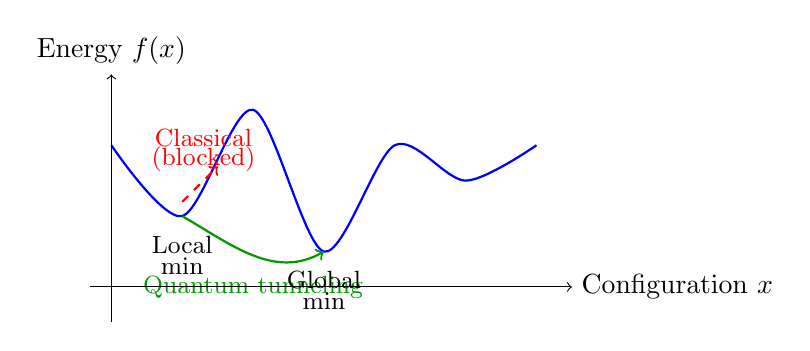
\begin{tikzpicture}[scale=0.9]
    % Energy landscape
    \draw[thick, blue] plot[smooth] coordinates {(0,2) (1,1) (2,2.5) (3,0.5) (4,2) (5,1.5) (6,2)};
    
    % Classical path (blocked)
    \draw[->, thick, red, dashed] (1,1.2) -- (1.5,1.7);
    \node[red] at (1.3,2.1) {\small Classical};
    \node[red] at (1.3,1.8) {\small (blocked)};
    
    % Quantum tunneling
    \draw[->, thick, green!60!black] (1,1) to[out=-30,in=210] (3,0.5);
    \node[green!60!black] at (2,0) {\small Quantum tunneling};
    
    % Labels
    \node at (1,0.6) {\small Local};
    \node at (1,0.3) {\small min};
    \node at (3,0.1) {\small Global};
    \node at (3,-0.2) {\small min};
    
    % Axes
    \draw[->] (-0.3,0) -- (6.5,0) node[right] {Configuration $x$};
    \draw[->] (0,-0.5) -- (0,3) node[above] {Energy $f(x)$};
\end{tikzpicture}
\caption{Quantum tunneling allows escaping local minima by passing through energy barriers.}
\end{figure}

\subsection{Tunneling in Optimization}

In the context of optimization:

\begin{itemize}
    \item \textbf{Local minima} are valleys in the energy landscape
    \item \textbf{Energy barriers} are the hills separating different valleys
    \item \textbf{Classical optimization} (like gradient descent) can get trapped in local minima
    \item \textbf{Quantum tunneling} provides a mechanism to escape local minima and find better solutions
\end{itemize}

\begin{keyconceptbox}[Advantage over Classical Methods]
Classical optimization methods escape local minima by:
\begin{enumerate}
    \item \textbf{Thermal excitation} (simulated annealing): Random jumps with probability $\propto e^{-\Delta E / k_B T}$
    \item \textbf{Momentum} (classical physics): Building up enough energy to ``roll over'' barriers
\end{enumerate}
Quantum tunneling offers a different mechanism: \textit{going through} barriers rather than over them. This can be exponentially faster for certain barrier shapes (thin, tall barriers).
\end{keyconceptbox}

\subsection{The Role of Transverse Field}

In quantum annealing, tunneling is enabled by a \textbf{transverse field} Hamiltonian:

\begin{equation}
    H_{\text{driver}} = -\sum_i X_i
\end{equation}

where $X_i$ is the Pauli-X operator. This creates superposition states that can ``tunnel'' between different configurations.

\begin{definitionbox}[Quantum Annealing Hamiltonian]
The total Hamiltonian in quantum annealing interpolates between driver and problem:
\begin{equation}
    H(s) = (1-s) H_{\text{driver}} + s H_P
\end{equation}
where $s$ goes from 0 to 1 during the anneal:
\begin{itemize}
    \item At $s=0$: System is in ground state of $H_{\text{driver}}$ (equal superposition)
    \item At $s=1$: System should be in ground state of $H_P$ (optimal solution)
\end{itemize}
\end{definitionbox}

\section{Adiabatic Theorem}
\label{sec:adiabatic}

The adiabatic theorem is the theoretical foundation guaranteeing that quantum annealing can find optimal solutions.

\begin{definitionbox}[Adiabatic Theorem]
If a quantum system starts in the ground state of an initial Hamiltonian $H_{\text{initial}}$, and the Hamiltonian is changed \textit{slowly enough} to a final Hamiltonian $H_{\text{final}}$, the system will remain in the instantaneous ground state throughout the evolution.
\end{definitionbox}

\textbf{The critical question:} How slow is ``slow enough''?

\begin{keyconceptbox}[Adiabatic Condition]
The evolution time $T$ must satisfy:
\begin{equation}
    T \gg \frac{\max_s |\bra{\psi_1(s)} \frac{dH}{ds} \ket{\psi_0(s)}|}{\min_s \Delta(s)^2}
\end{equation}
where $\Delta(s) = E_1(s) - E_0(s)$ is the \textbf{minimum spectral gap} between ground and first excited state.

\textbf{Implication:} Small gaps require long evolution times. If the gap closes (becomes zero), adiabatic evolution fails.
\end{keyconceptbox}

\begin{warningbox}[Gap Problem]
For hard optimization problems, the spectral gap can become exponentially small, requiring exponentially long anneal times. This is analogous to phase transitions in statistical physics where the correlation length diverges.
\end{warningbox}

\subsection{Adiabatic Quantum Computing}

The adiabatic theorem leads to a model of quantum computation:

\begin{enumerate}
    \item \textbf{Encode} the problem in $H_P$ (problem Hamiltonian)
    \item \textbf{Initialize} in ground state of easy $H_{\text{driver}}$
    \item \textbf{Evolve} slowly: $H(t) = (1 - t/T) H_{\text{driver}} + (t/T) H_P$
    \item \textbf{Measure} to obtain the solution
\end{enumerate}

\begin{notebox}
Adiabatic quantum computing is computationally equivalent to gate-model quantum computing. Any problem solvable by one can be solved by the other with polynomial overhead.
\end{notebox}

\begin{tipbox}[Relevance to Image Segmentation]
Quantum annealing exploits tunneling to solve QUBO formulations of image segmentation. The image segmentation objective (data fidelity + smoothness) is encoded as $H_P$. The quantum annealer then finds low-energy configurations---which correspond to good segmentations---by tunneling through the complex energy landscape of possible pixel labelings.
\end{tipbox}
